% !TEX root = ../Grunddatei.tex
\section{Versuchsaufbau und Versuchsdurchführung}

\subsection{Kennlinie des aktiven Zweipols}
Der Versuchsaufbau besteht aus einer Spannungsquelle, zwei Multimetern zur Spannungs- bzw. Strommessung, und einem Schiebewiderstand. Der Versuchsaufbau ist in Abbildung \ref{fig:versuchsaufbau} dargestellt.
\begin{figure}[ht]
    \centering
    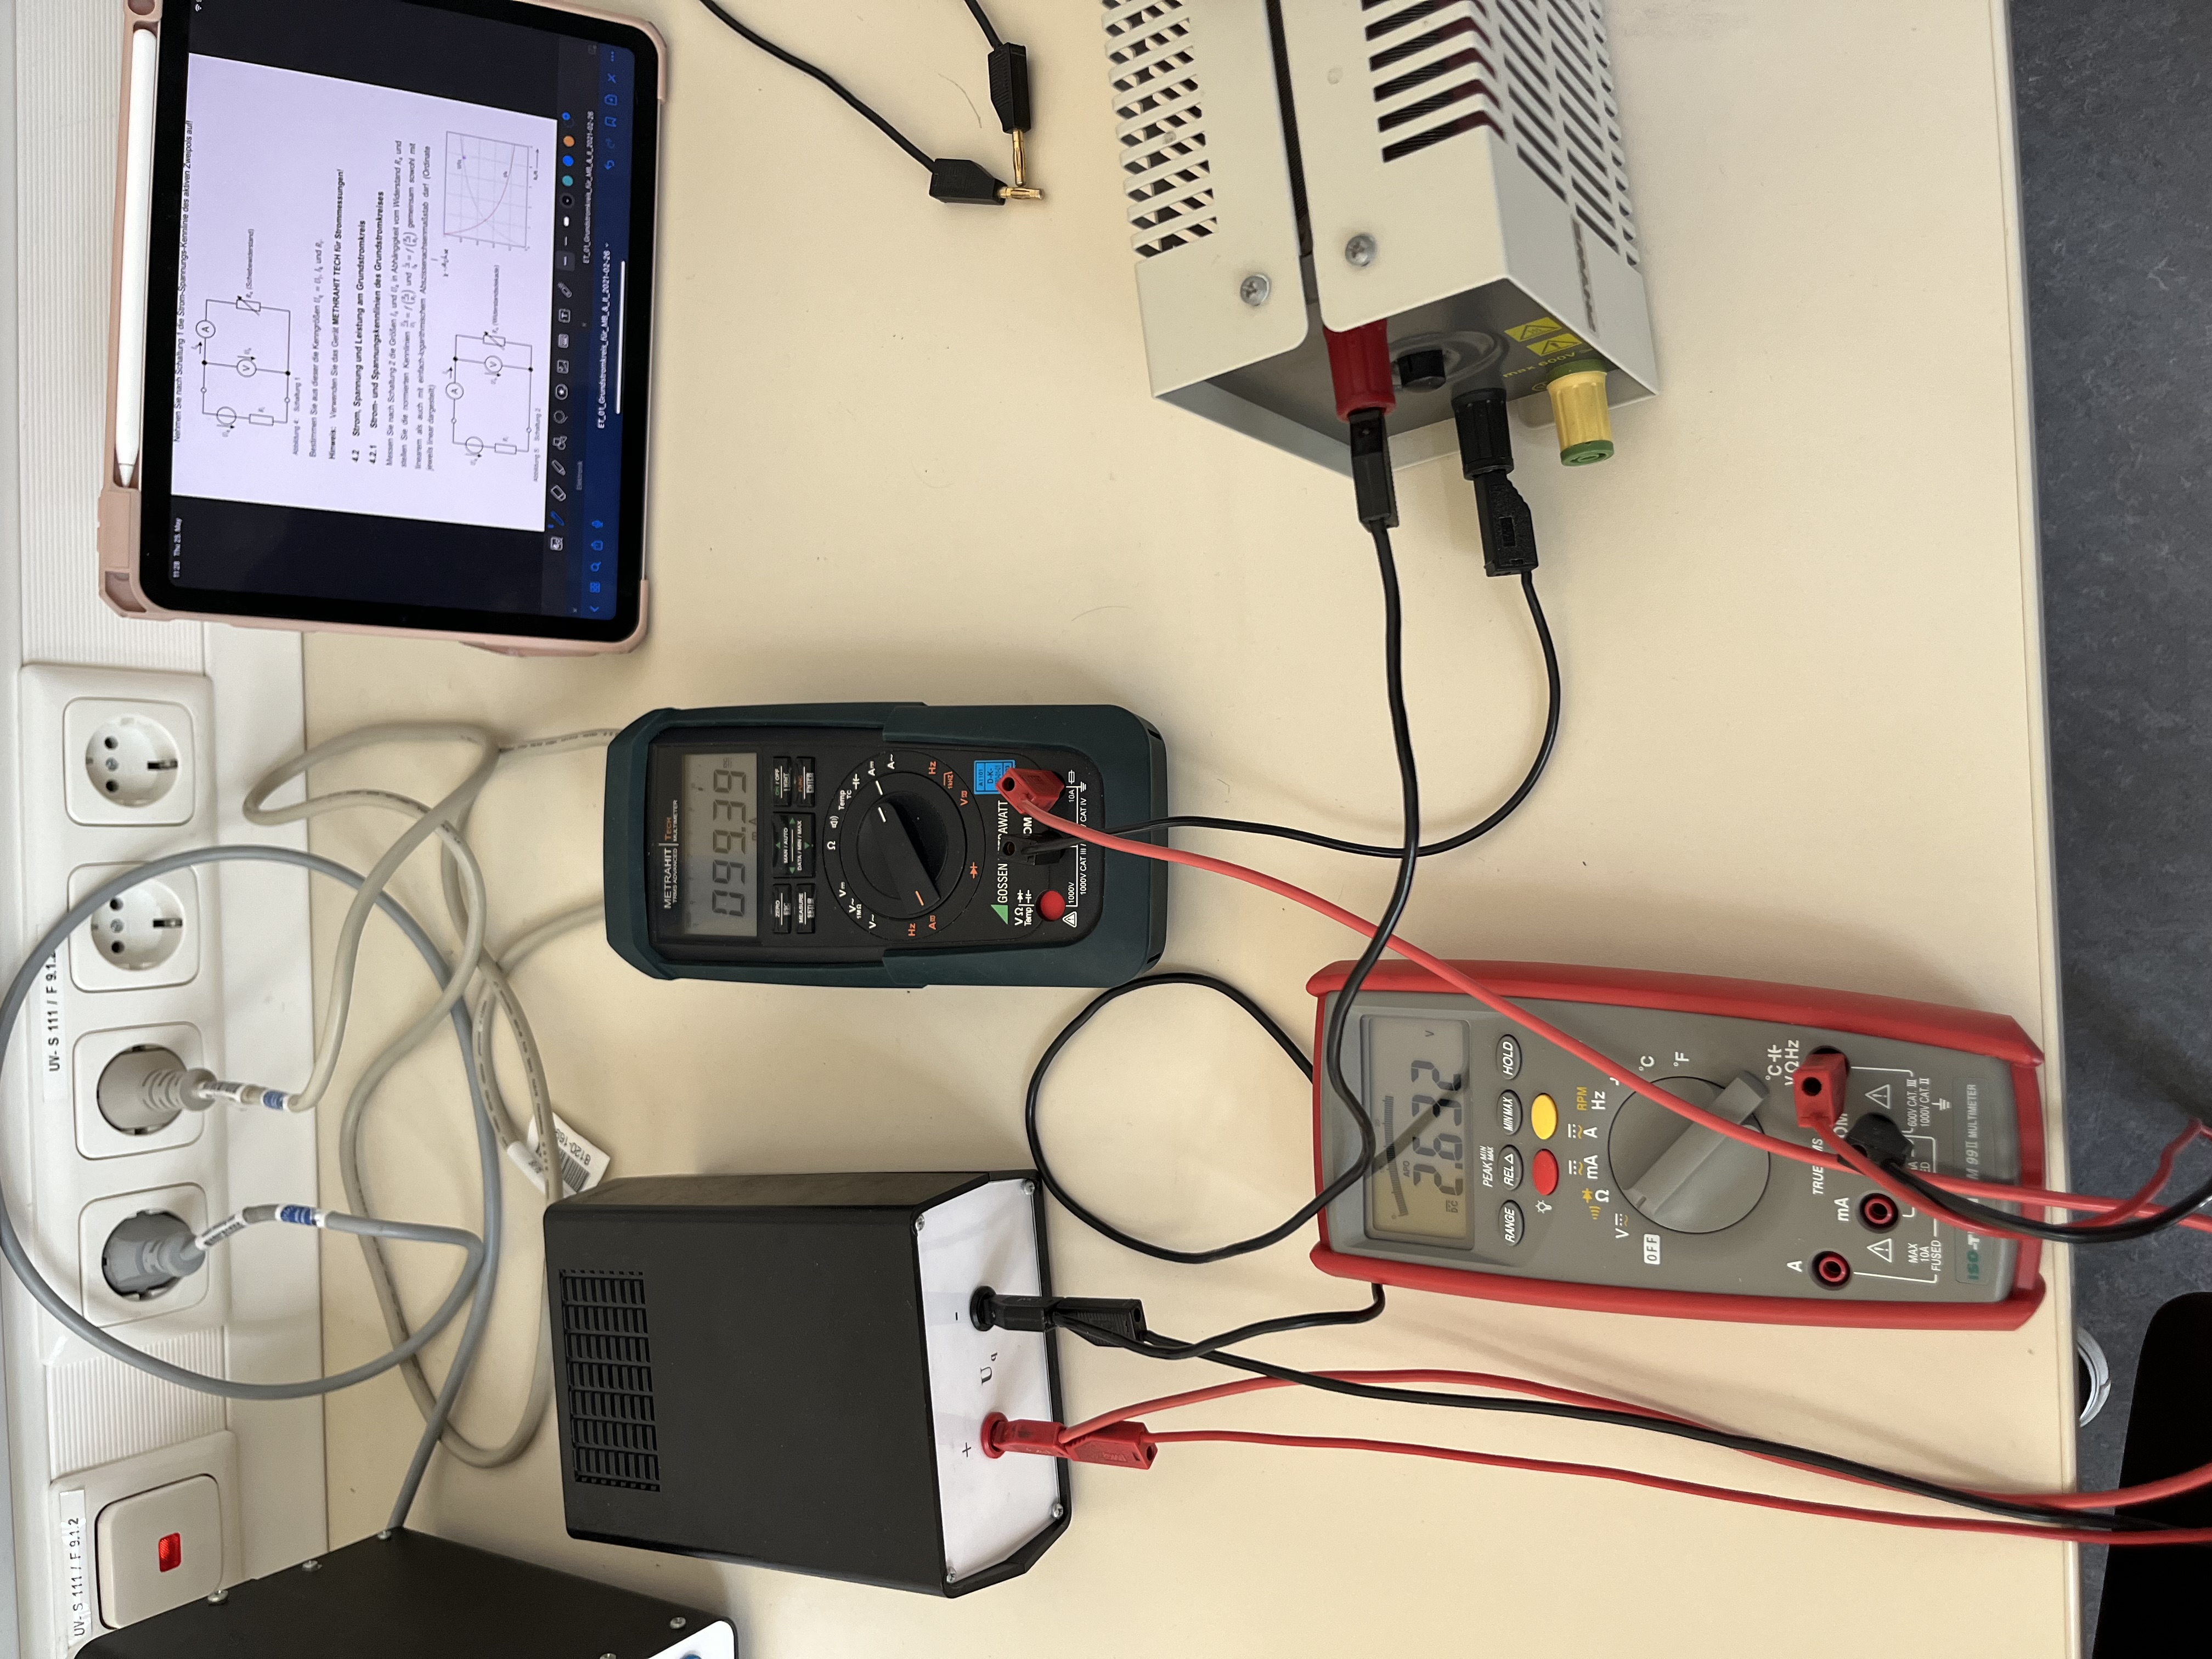
\includegraphics[width=0.5\linewidth]{Bilder/Versuchsaufbau.png}
    \caption{Versuchsaufbau aktiver Zweipol}
    \label{fig:versuchsaufbau}
\end{figure}

Zuerst wird $R_a=0\,\Omega$ eingestellt, um den Kurzschlussstrom $I_k$ zu messen. Dann wird der Schiebewiderstand aus der Schaltung abgeklemmt. Dadurch wird die Leerlaufspannung $U_l$ gemessen.
Es ergeben sich die Werte
\begin{align*}
    I_k & = 2,67\,A  \\
    U_l & = 8\,V\, .
\end{align*}

\subsection{Strom-Spannungs-Kennlinie des Grundstromkreises}

Für verschiedene Widerstände $R_a$ werden nun die Spannung und der Strom gemessen. Die Messwerte sind in Tabelle \ref{tab:aktiveZweipole} zu sehen. Zu jedem Messwertpaar kann der Wirkungsgrad $\eta$ berechnet und in die Tabell eingetragen werden. Dieser ist definiert als
\begin{equation*}
    \label{eq:wirkungsgrad}
    \eta = \frac{R_a}{R_i+R_a}
\end{equation*} mit $R_i = 3\,\Omega$ aus der Versuchsvorbereitung. Außerdem wird die abgegebene Leistung $P_a$ nach \eqref{eq:abgegebeneLeistungAllgemein} berechnet und in die Tabelle eingetragen.
\begin{center}
    \begin{table}[ht]
        \begin{tabularx}{\linewidth}{|*{5}{X|}}
            \hline
            $R_a$/\,$\Omega$ & $U_{AB}$/\,V & $I$/\,mA & ${\eta}$ & $P_a$/\,mW \\
            \hline
            3                & 0,63         & 182,4    & 0,11     & 114        \\
            6                & 1,06         & 164,4    & 0,2      & 174        \\
            12               & 1,71         & 137,5    & 0,33     & 235        \\
            24               & 2,47         & 101,2    & 0,5      & 250        \\
            48               & 3,31         & 68,2     & 0,67     & 226        \\
            96               & 3,98         & 41,3     & 0,8      & 164        \\
            192              & 4,44         & 23,1     & 0,89     & 103        \\
            384              & 4,71         & 12,3     & 0,94     & 58         \\
            \hline
        \end{tabularx}
        \caption{Messwerte und Berechnungen im aktiven Zweipol}
        \label{tab:messwerteAktiverZweipol}
    \end{table}
\end{center}

Mit den Kenngrößen $U_l=5,02\,$V und $I_k=208\,$mA des aktiven Zweipols lässt sich die maximale Leistung, die der aktive Zweipol abgeben kann, berechnen. Diese ist gegeben durch
\begin{equation*}
    P_{a,max} = U_l \cdot I_k = 1,04\,W\, .
\end{equation*}

In den Diagrammen \ref{fig:stromSpannungsKennlinie} und \ref{fig:leistungWirkungsgrad} sind die Messwerte graphisch dargestellt. In Abbildung \ref{fig:stromSpannungsKennlinie} sind die normierten Kennlinien $\frac{U_a}{U_l}=f\left(\frac{R_a}{R_i}\right)$ und $\frac{I}{I_k}=f\left(\frac{R_a}{R_i}\right)$, in Abbildung \ref{fig:leistungWirkungsgrad} die nach der Maximalleistung normierte abgegebene Leistung $\frac{P_a}{P_{a,max}}=f\left(\frac{R_a}{R_i}\right)$ sowie der Wirkungsgrad $\eta=f\left(\frac{R_a}{R_i}\right)$ dargestellt.

\begin{figure}[ht]
    \begin{subfigure}[h]{0.4\linewidth}
        \includegraphics[width=\linewidth]{example-image-a}
        \caption{Strom und Spannung}
        \label{fig:stromSpannungsKennlinie}
    \end{subfigure}
    \hfill
    \begin{subfigure}[h]{0.4\linewidth}
        \includegraphics[width=\linewidth]{example-image-b}
        \caption{Leistung und Wirkungsgrad}
        \label{fig:leistungWirkungsgrad}
    \end{subfigure}
    \caption{Darstellung in Abhängigkeit von $R_a$}
\end{figure}

\subsection{Analyse eines Netzwerkes}
Der Versuchsaufbau entspricht dem in Abbildung \ref{fig:versuchsaufbauNetzwerk} zu sehenden Aufbau und besteht aus drei Spannungsquellen, vier Widerständen sowie einem Multimeter zur Spannungs-, Strom- und Widerstandsmessung.
\begin{figure}[ht]
    \centering
    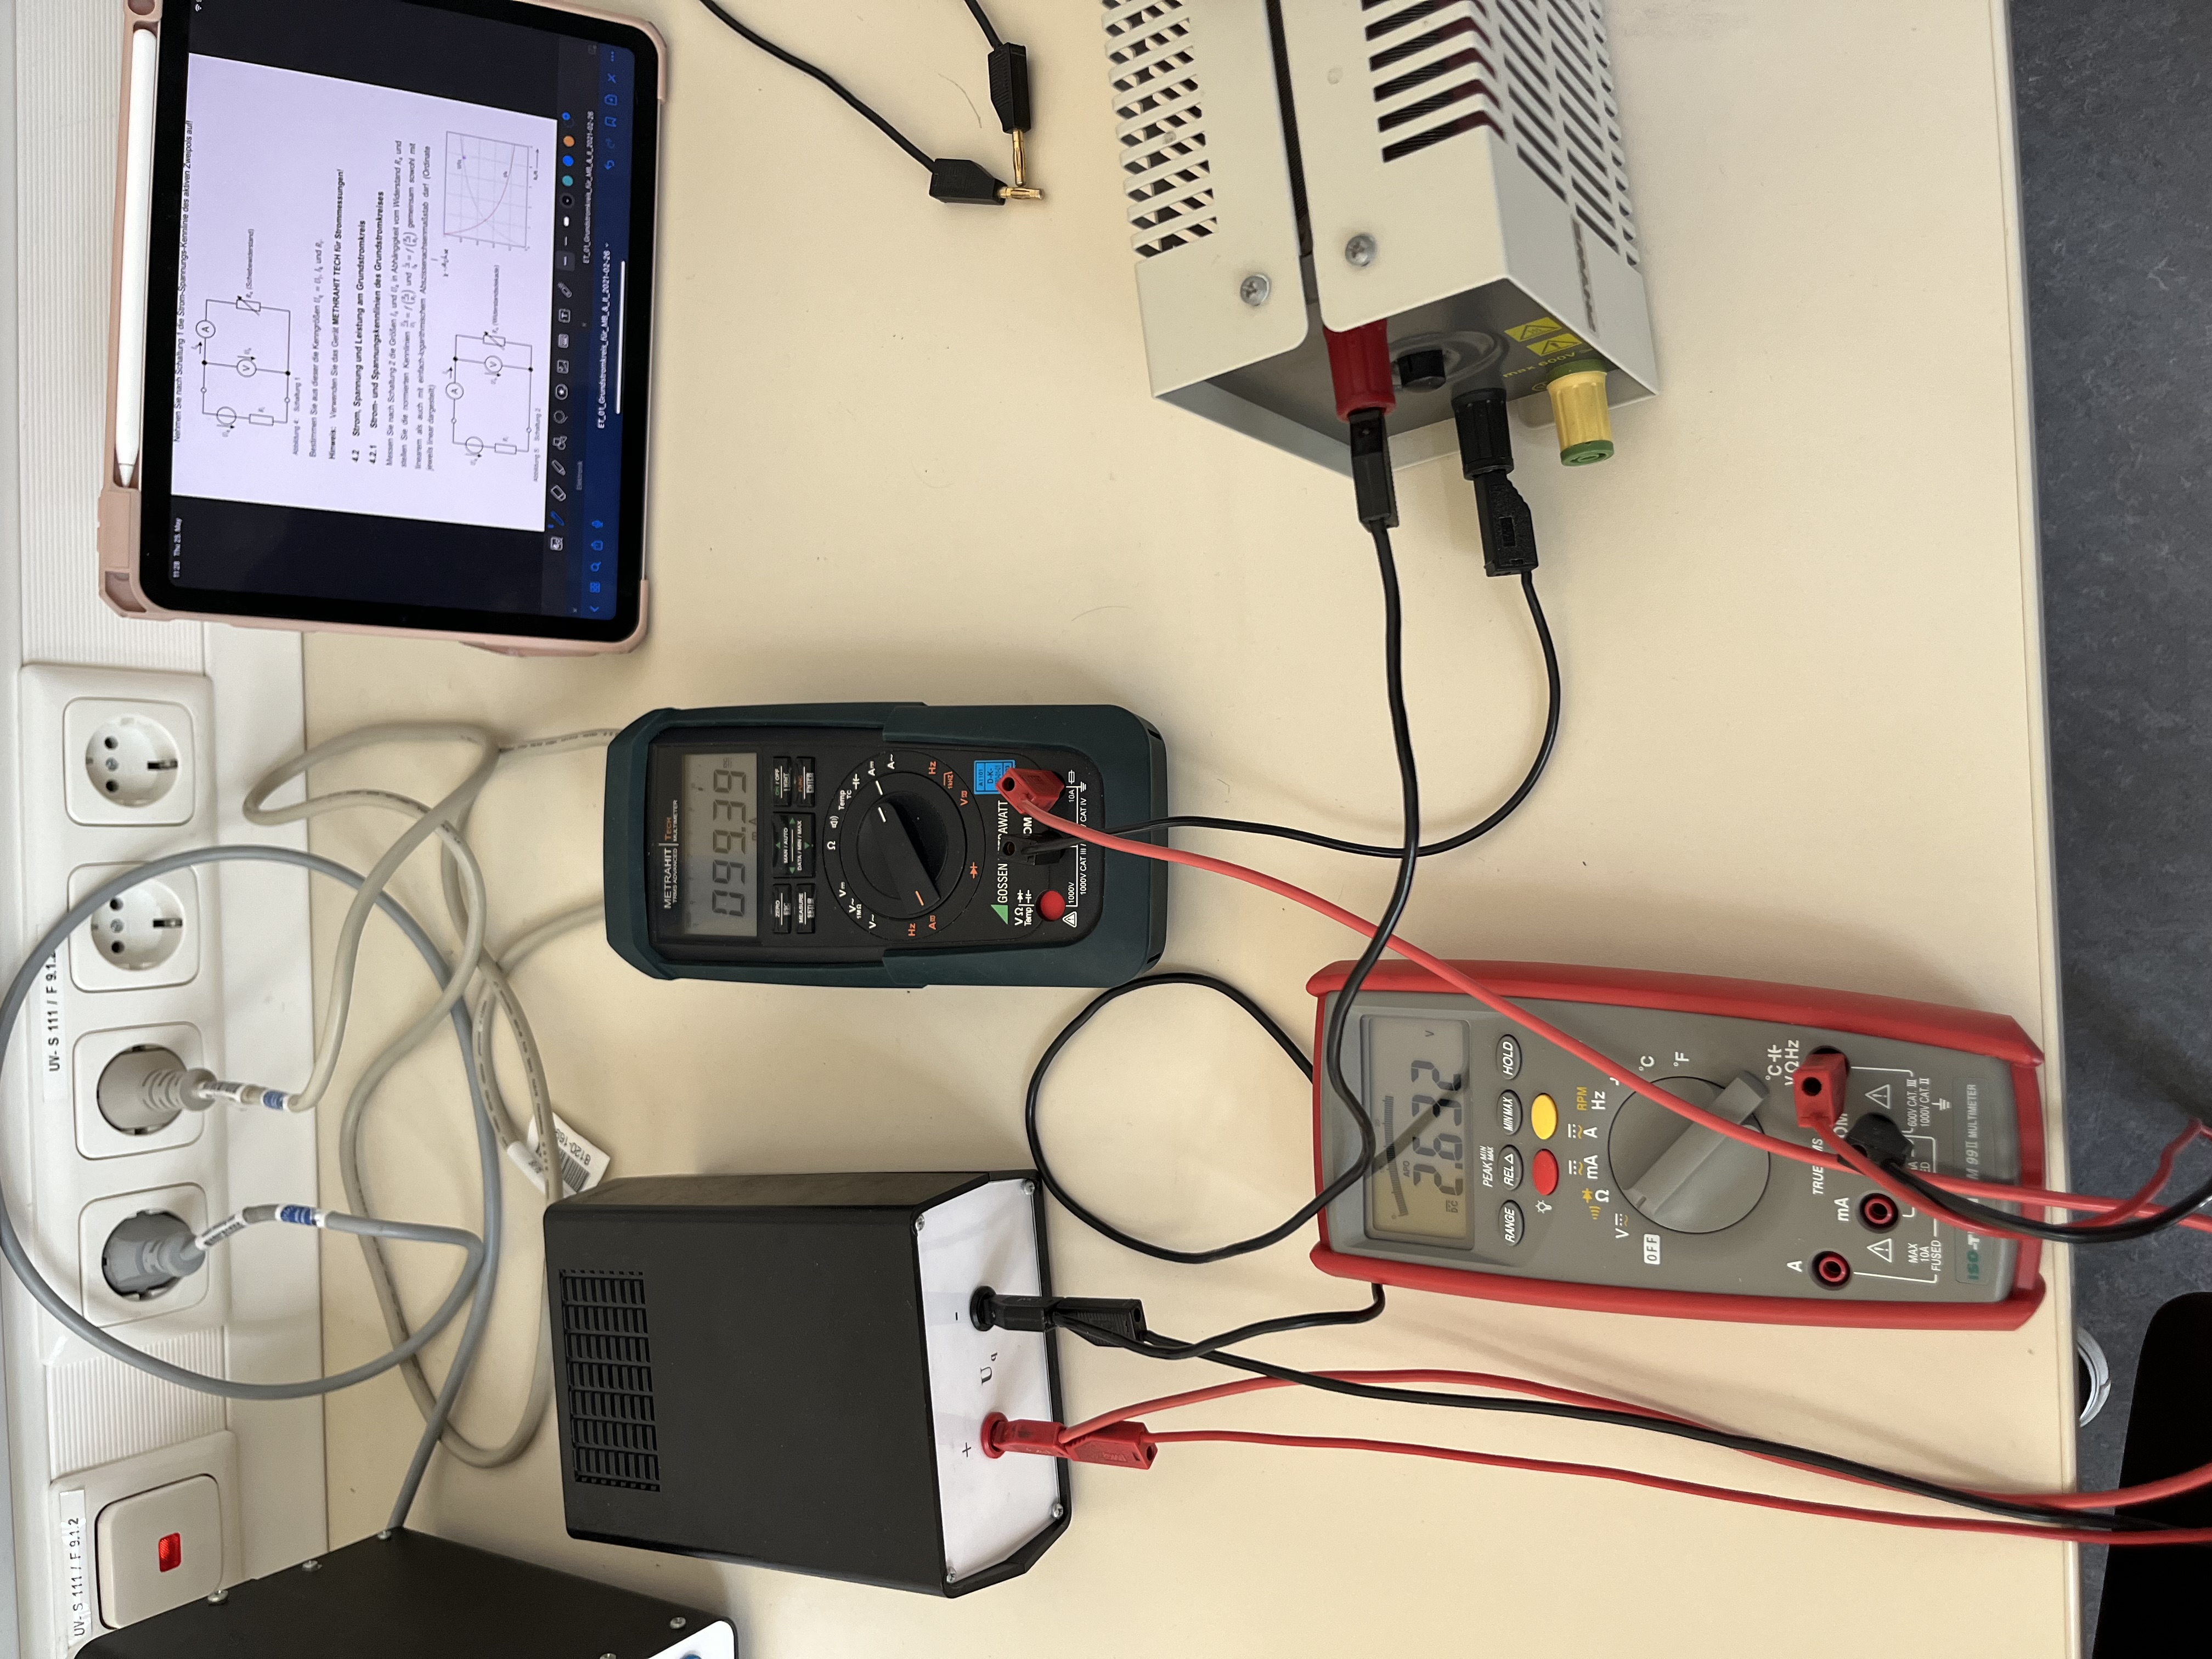
\includegraphics[width=0.5\linewidth]{Bilder/Versuchsaufbau.png}
    \caption{Versuchsaufbau}
    \label{fig:versuchsaufbauNetzwerk}
\end{figure}

\subsection*{Widerstände}
Zuerst werden mit dem Multimeter die Widerstände der Widerstände $R_1$, $R_2$, $R_3$ und $R_4$ gemessen. Es ergeben sich die Werte
\begin{align*}
    R_1 & = 820\,\Omega \\
    R_2 & = 558\,\Omega \\
    R_3 & = 525\,\Omega \\
    R_4 & = 678\,\Omega
\end{align*}
sowie ein Ersatzinnenwiderstand $R_{i,ers}$ bei überbrückten Quellspannungen von
\begin{align*}
    R_{i,ers} & = 1055\,\Omega\, .
\end{align*}

Der berechnete Ersatzinnenwiderstand $R_{i,ers,berechnet}$ beträgt
\begin{align*}
    R_{i,ers,berechnet} & = \left(R_1+R_2\right)\parallel{R_3+R_4}\,\Omega\,
    = 1058\,\Omega\, .
\end{align*}

\subsection{Quellspannungen}
Die Quellspannungen $U_{q1}$, $U_{q2}$ und $U_{q3}$ werden mit dem Multimeter gemessen. Es wurden die Werte
\begin{align*}
    U_{q1} & = -8,03\,V \\
    U_{q2} & = 11,14\,V \\
    U_{q3} & = 10,26\,V
\end{align*}
sowie eine Leerlaufspannung $U_{l,AB}$ von
\begin{align*}
    U_{l,AB}=8,28\,V\,
\end{align*}
gemessen.

\subsection{Zweigstrom $I_{AB}$}
Analog zum Vorgehen in der Vorbereitung (\ref{sec:helmholtz}) wird der Zweigstrom $I_{AB}$ berechnet. Dazu wird jeweils eine Spannungsquelle verwendet und die anderen beiden überbrückt. Zunächst erfolgt die theoretische Berechnung des Zweigstroms $I_{AB}$ mit den Widerständen $R_1$, $R_2$, $R_3$ und $R_4$ sowie den Quellspannungen $U_{q1}$, $U_{q2}$ und $U_{q3}$. Es ergibt sich für $U_{q1}$ zunächst der Gesamtwiderstand $R_{ges1}$ zu
\begin{equation*}
    R_{ges1}=R_1+R_2+(R_3\parallel R_4)=1674\,\Omega\, ,
\end{equation*}
dadurch der Gesamtstrom $I_{1}$ mit
\begin{equation*}
    I_{1}=\frac{U_{q1}}{R_{ges1}}=-4,80\,mA
\end{equation*}
und schließlich der Zweigstrom $I_{AB1}$
\begin{equation}
    \label{eq:zweigstrom1}
    I_{AB1}=\frac{R_3}{R_3+R_4}\cdot I_{1}=-2,1\,mA\, .
\end{equation}

Analog wird für $U_{q2}$ der Gesamtwiderstand $R_{ges2}$ zu
\begin{equation*}
    R_{ges2}=R_1+(R_2\parallel R_3)+R_4=1674\,\Omega\, ,
\end{equation*}
der Gesamtstrom $I_{2}$ mit
\begin{equation*}
    I_{2}=\frac{U_{q2}}{R_{ges2}}=6,7\,mA
\end{equation*}
und schließlich der Zweigstrom $I_{AB2}$
\begin{equation}
    \label{eq:zweigstrom2}
    I_{AB2}=\frac{R_3}{R_3+R_4}\cdot I_{2}=2,9\,mA\,
\end{equation}
berechnet.

Zum Schluss ergibt sich für $U_{q3}$ mit dem Gesamtwiderstand $R_{ges3}$ zu
\begin{equation*}
    R_{ges3}=R_3+(R_1+R_2)\parallel{R_4}=979\,\Omega\, ,
\end{equation*} und $I_{3}=10,4\,mA$ schließlich der Zweigstrom $I_{AB3}$
\begin{equation}
    \label{eq:zweigstrom3}
    I_{AB3}=\frac{R_1+R_2}{R_1+R_2+R_4}\cdot I_{3}=7\,mA\, .
\end{equation}

Als Gesamtzweigstrom ergibt sich damit durch Addition der einzelnen Zweigströme {\eqref{eq:zweigstrom1}}, {\eqref{eq:zweigstrom2}} und {\eqref{eq:zweigstrom3}} der Wert
\begin{equation}
    I_{AB}=I_{AB1}+I_{AB2}+I_{AB3}=7,8\,mA\, .
\end{equation}

Überprüft man diese Werte mit dem Multimeter, so ergeben sich die Werte
\begin{align*}
    I_{AB1} & = -2,1\,mA    \\
    I_{AB2} & = 2,9\,mA     \\
    I_{AB3} & = 7,0\,mA     \\
    I_{AB}  & = 7,8\,mA\, .
\end{align*}
Es ist zu sehen, dass die gemessenen Werte mit den berechneten Werten übereinstimmen.




